%\documentclass[11pt,dvipdfm]{article}
\documentclass[11pt]{article} %The above line must be used for your camera-ready submission, which requires a latex -> DVI -> PDF compilation pipeline.  As a workaround while you are writing your paper, you could comment it out and use this line instead, which is compatible with pdflatex.

%\documentclass[conference,onecolumn]{IEEEtran}
% \IEEEoverridecommandlockouts
% The preceding line is only needed to identify funding in the first footnote. If that is unneeded, please comment it out.
\usepackage{deauthor,times}


%\usepackage{tabularx}
\usepackage{booktabs}
%\usepackage[super]{nth}     % for easier ordinal number
\usepackage{enumitem}     % better lists
\usepackage{url}
\usepackage{hyperref}
\usepackage{multicol}
\usepackage{footnote}
%\usepackage{cite}
%\usepackage{graphicx}
\usepackage{xcolor}
\def\BibTeX{{\rm B\kern-.05em{\sc i\kern-.025em b}\kern-.08em
    T\kern-.1667em\lower.7ex\hbox{E}\kern-.125emX}}
    
%\usepackage{amsmath,amssymb,amsfonts}
%\usepackage{algorithmic}
%\usepackage{textcomp}

\definecolor{darkgray}{RGB}{100,100,100}
\definecolor{darkplum}{RGB}{50,10,50}
\definecolor{Mahogany}{RGB}{103,10,10}
\definecolor{RedInstruct}{RGB}{180,45,45}

% QUOTE AFFILIATIONS
\newcommand\aff[1]{\textcolor{darkplum}{{\emph{--#1}}}}

% QUESTION LABELS
% flip the next two lines to turn on and off question labels
% \newcommand\q[1]{\textcolor{Mahogany}{\small{\textbf{[#1]}}}}
  \newcommand\q[1]{\textcolor{Mahogany}{\small{\textbf{}}}}

% tables for grayness
\newcommand\graynew[1]{\textcolor{darkgray}{#1}}

% FORMATTING FOR OUR QUOTE LISTS

\newenvironment{lq2}
{ \vspace{-3pt}
  \begin{itemize}[leftmargin = 4.0em, rightmargin=5.0em, label={}]
    \fontsize{10pt}{10.7pt}\selectfont
    \setlength{\itemsep}{3pt}
    \setlength{\parskip}{2.5pt}
    \setlength{\parsep}{3pt}     }
{ \end{itemize} \vspace{1pt}  }

% FORMATTING FOR OUR QUOTE LISTS IN THE FIGURE PAGE

\newenvironment{lq1}
{ \begin{itemize}[leftmargin = 0em, label={}]
    \fontsize{8pt}{8.6pt}\selectfont
    \setlength{\itemsep}{2pt}
    \setlength{\parskip}{2pt}
    \setlength{\parsep}{2pt}       }
{ \end{itemize}                    }

% MACRO FOR GROUP LABELS

 \def\Exciting/{{\fontfamily{lmss}\selectfont\textbf{Exciting}}}  \def\Useful/{{\fontfamily{lmss}\selectfont\textbf{Useful}}}
 \def\Worrying/{{\fontfamily{lmss}\selectfont\textbf{Worrying}}}
 \def\Futuristic/{{\fontfamily{lmss}\selectfont\textbf{Futuristic}}}
 \def\None/{{\fontfamily{lmss}\selectfont\textbf{None}}}

%\newcommand{\highlight}{\cellcolor{lightgray}}

% MACROS FOR QUESTIONS IN THE SUPPLEMENT
% \newcommand\question[1]{\bigskip\noindent\textcolor{darkgray}{\large{\textbf{#1}}}\newline}
\newcommand\question[1]{\bigskip\noindent\textcolor{darkgray}{{\textbf{#1}}}\newline}
\newcommand\sample[1]{\noindent\{\textcolor{RedInstruct}{#1}\}\newline}
\newcommand\questiontext[1]{\noindent{#1}}
\newcommand\openend{\\[2pt]\indent\{Open-end\}}





\begin{document}
\title{``Mixture of amazement at the potential of this technology and concern about possible pitfalls'': Public sentiment towards AI in 15 countries}
\author{
  Patrick Gage Kelley,* Yongwei Yang,* Courtney Heldreth,* \\
  Christopher Moessner,$\dagger$ Aaron Sedley,* Allison Woodruff* \vspace{0.2cm}\\ 
  ~*\textit{Google} \\
        \fontfamily{pcr}\selectfont\small
        \href{mailto:patrickgage@acm.org}{patrickgage@acm.org},
        \href{mailto:yongwei@google.com}{yongwei@google.com},
        \href{mailto:cheldreth@google.com}{cheldreth@google.com}, \\ 
        \fontfamily{pcr}\selectfont\small
        \href{mailto:asedley@google.com}{asedley@google.com}, 
        \href{mailto:woodruff@acm.org}{woodruff@acm.org} \vspace{0.2cm}\\
  $\dagger$\textit{Ipsos}\\
        \fontfamily{pcr}\selectfont\small
        \href{mailto:christopher.moessner@ipsos.com}{christopher.moessner@ipsos.com}}





\maketitle

\begin{abstract}
Public opinion plays an important role in the development of technology, influencing product adoption, commercial development, research funding, career choices, and regulation. In this paper we present results of an in-depth survey of public opinion of artificial intelligence (AI) conducted with over 17,000 respondents spanning fifteen countries and six continents. Our analysis of open-ended responses regarding sentiment towards AI revealed four key themes (exciting, useful, worrying, and futuristic) which appear to varying degrees in different countries. These sentiments, and their relative prevalence, may inform how the public influences the development of AI.

\end{abstract}

%\begin{IEEEkeywords}
%artificial intelligence, public opinion, survey research
%\end{IEEEkeywords}

\section{Introduction}
Increased understanding of the societal impact of artificial intelligence (AI) has spurred strong interest its in responsible development~\cite{dietterich2015rise,hawking2014,horvitz2012interim, stone2016artificial}.
Researchers, advocates, companies, and others have proposed processes, principles, design toolkits, and other resources to support thoughtful development of AI that carefully considers both benefits and risks~\cite{abrassart2018, fjeld2020, highlevel2019,jobin2019,scuEthics,googleAI,princetonEthics,ethicalOS}.

Public opinion is an important force in responsible development, exerting pressure on funding agencies, regulators, companies, educators, and others to address both general attitudes and specific issues~\cite{castro2019, cave2018portrayals,ouchchy2020,zhang2022}, such as the impact of automation on the future of work~\cite{brynjolfsson2014second, raghavan2020, sanchez-mondero2020},  the interaction of AI with human rights issues such as privacy and discrimination~\cite{abrassart2018, barabas2018, buolamwini2018, chancellor2019}, the ethics of autonomous weapons~\cite{scharre2018army, west2018}, and the development and availability of dual-use technologies such as synthetic media that may be used for either benevolent or nefarious purposes~\cite{openAI2019}. While public opinion may not fully align with expert assessment on these issues, it is nonetheless useful to elucidate the forces in effect.

 While there have been some explorations of public perception of AI, for example, survey research~\cite{arm2017, blumberg2019, cave2019, ipsos2019, mozilla2019, northeastern2018, west2018, zhang2019artificial}, sentiment analysis~\cite{chuan2019, fast2017long, garvey2019sentiment, ouchchy2020}, and narrative analysis~\cite{cave2018portrayals, cave2020narratives}, much of this work has been done in Western, English-speaking contexts. Even in these better studied contexts, much remains to be learned, as both the technology and the public discussion are evolving rapidly. In this paper, we present a survey of public perception of AI conducted with over 17,000 respondents spanning fifteen countries and six continents (encompassing in total: Germany, Australia, Finland, Singapore, Belgium, Canada, the United States (US), South Korea, Spain, France, Poland, Brazil, China, India, and Nigeria). Using an inductive approach to analyze open-ended responses, we identified four key sentiment groups (exciting, useful, worrying, and futuristic) whose prevalence distinguishes responses to AI in different countries. We previously shared results from eight of these countries~\cite{kelley2021} and here we extend our analysis to fifteen countries and more fully discuss the sentiments. We then discuss implications of these findings for the development of AI systems. 

\section{Background}
Artificial intelligence (AI) is a broad term with no consensus definition~\cite{edelman2019, fast2017long, stone2016artificial},
and the scope of our inquiry is intended to be similarly broad.
We note that interpretation of the term is further confounded by the ``AI effect'' (the phenomenon that once AI successfully solves a problem and the solution becomes commonplace, it is no longer considered to be AI)~\cite{mccorduck2004machines}, as well as lack of awareness of algorithmic processing in common systems~\cite{eslami2015always, rader2015understanding, warshaw2016intuitions}. 
To aid comparison with survey responses,
following~\cite{stone2016artificial}, we share with the reader the following definition provided by Nils J. Nilsson: ``Artificial intelligence is an activity devoted to making machines intelligent, and intelligence is the quality that enables an entity to function appropriately and with foresight in its environment.''~\cite{nils2009}

\subsection{Empirical Studies}
Much of the research on public perception of AI has been survey-based, often conducted in Western, English-speaking countries such as the US and the UK~\cite{blumberg2019, cave2019, edelman2019, zhang2019artificial, northeastern2018} although this has been broadening recently.
AI is often viewed as likely to have a significant impact on the future, with a frequent expectation that its effects will be positive.
In a 2019 Edelman survey in the US, 9 out of 10 respondents assumed that AI will be life-changing and transformational~\cite{edelman2019}.
A Gallup survey conducted in the US in 2018 found that 76\% believed that AI will have a positive impact on their lives~\cite{northeastern2018}; 61\% of respondents had a positive view of AI and robots in a large-scale 2017 survey across Europe on the impact of digitization and automation on daily life~\cite{european2017}; and a 2017 consumer research survey conducted across North America, Europe, and Asia revealed a predominant expectation that society will become better (61\%) rather than worse (22\%) due to increased automation and AI~\cite{arm2017}. A recent Pew Research survey conducted across the Americas, Europe, and Asia showed a somewhat narrower margin (possibly due to shifting public opinion, or alternatively, methodological differences), with a median of 53\% saying that AI has been mostly good for society (53\%) versus mostly bad (33\%)~\cite{funk2020}. Considering expected impact in the next 20 years, the 2019 World Risk Poll indicated AI would mostly help (41\%) versus mostly harm (30\%) people in one's own country, with more favorable impressions in Asia and less favorable impressions in Western countries~\cite{lloyds2020, neudert2020}.

At the same time, AI is neither interpreted as exclusively beneficial nor exclusively disadvantageous, and public response often indicates contradictory emotions. Looking at broad reactions, Blumberg reported that US respondents were equally split between feeling optimistic and informed and feeling fearful and uninformed about AI~\cite{blumberg2019}, while~\cite{arm2017} also revealed both excitement and concern. Relatedly, a 2019 Mozilla survey open to respondents on the Internet gathered continent-level demographic data and revealed varying and mixed emotions at the continent-level~\cite{mozilla2019}. Specific concerns have been expressed regarding social issues, such as AI benefiting the wealthy and harming the poor, fear that AI-enabled deepfakes will erode trust in information, and AI increasing social isolation and reducing human capability~\cite{edelman2019}. In line with these concerns, Zhang and Dafoe found that 82\% of Americans want AI and robots to be carefully managed~\cite{zhang2019artificial}, with 88\% of Europeans expressing similar sentiment~\cite{european2017}. Moreover, 60\% of the general population in the Edelman survey expressed the need for more regulation regarding AI development and deployment~\cite{edelman2019}.

Qualitative work has also explored public perception of algorithmic systems, for example, finding that perception of algorithmic systems can vary substantially by individual factors as well as platform~\cite{devito2017platforms}, and that end users often have fundamental questions or misconceptions about technical details of their operation~\cite{bucher2017algorithmic, eslami2015always, rader2015understanding, ur2012smart, warshaw2016intuitions}.

\subsection{Narratives and Media Sentiment Analysis}
AI is not only heavily discussed in academia, but is also a popular topic in public media and entertainment~\cite{edelman2019}. In fact, Cave et al. provide a history of narratives about intelligent machines dating back to ancient Greece~\cite{cave2020narratives}. In modern times, 58\% of the respondents in a recent Blumberg survey indicated that they get information about AI from movies, TV, and social media~\cite{blumberg2019}. In a 2016 CBS news survey, only 19\% indicated not having seen any of several AI movies such as ``The Terminator'' or ``I, Robot''~\cite{cbs2016}. Cave et al. argue that prevalent AI narratives in the English-speaking West share ``a tendency towards utopian or dystopian extremes,'' cautioning that inaccurate narratives could affect technological advancement and regulation~\cite{cave2018portrayals}, with similar points raised in~\cite{horvitz2012interim, stone2016artificial, you2015}. Cave et al. surveyed UK respondents regarding their responses to eight dominant narratives about AI, reporting that the strong majority elicited more concern than excitement~\cite{cave2019}.

At the same time, while some researchers have argued that narratives and fiction may be disproportionately frightening, studies have suggested that news reports may be more balanced or appropriately critical. Sentiment analysis of newspaper articles from the New York Times and associated content found that, in general, AI has had consistently more optimistic than pessimistic coverage over time~\cite{fast2017long}, and did not support the hypothesis that news media coverage of AI is negative~\cite{garvey2019sentiment}. Content analysis of coverage of AI in five major American newspapers revealed benefits were discussed more frequently than risks, although risks were discussed with greater specificity~\cite{chuan2019}. Ouchchy et al. analyzed discussion of AI ethics in English language media sources and concluded that ``The issues most frequently covered, along with the mostly balanced/neutral tones, suggest that the media has a fairly realistic and practical focus in its coverage of the ethics of AI.''~\cite{ouchchy2020}

\subsection{National Considerations}
A number of countries have established national strategies to promote the use and development of AI, which vary by country and may influence public perception~\cite{dutton2018}.\footnote{See also \url{https://futureoflife.org/national-international-ai-strategies/}} 
The importance of studying local context is also illustrated by analysis of country-specific opportunities and challenges for AI, e.g.~\cite{kalyanakrishnan2018opportunities}.
Further, researchers have called for better integration of developing country considerations in the discussion and development of AI~\cite{sambasivan2019toward}.

\subsection{Our Approach}
Our work sits within a growing body of research on people’s perceptions of AI, across disciplines including HCI, critical studies, law, marketing, policy, psychology, and more. This topic is highly complex, multi-dimensional, and far from fully understood. Methodologically, this means that techniques such as \textit{triangulation} (studying the same phenomenon from multiple vantage points, in order to cross-check and more fully capture richness and complexity, e.g. using both qualitative and quantitative methods to see if the findings are consistent)~\cite{salkind2010} and \textit{replication} (the reproduction and extension of prior work)~\cite{wilson2014} are particularly useful for this topic. Accordingly, we seek to broaden and enrich the understanding of sentiment towards AI by looking for emergent themes in a large number of open-ended responses from a wide range of countries.


\section{Methodology}
In order to better understand public perception of AI, 
we partnered with Ipsos, a global market research firm, 
to conduct a survey of 17,014 respondents in fifteen countries in July and December 2019.\footnote{For logistical reasons we split data collection into two rounds: July 2019 (Australia, Canada, US, South Korea, France, Brazil, India, and Nigeria) and December 2019 (Germany, Finland, Singapore, Belgium, Spain, Poland, and China). Based on our experience with similar surveys and our knowledge of world events at the time, we do not expect the time interval between the two rounds had a substantial impact on the results.}
Methodologically, this work falls in the genre of public opinion polling, as described below.

\subsection{Instrument Development and Translation}
To develop concepts and questions, we consulted experts at our institutions, reviewed published work, drew on our own previous unpublished research, and conducted an initial pilot survey in June 2018 with 1300 respondents drawn from a panel of the general online population in the US. Many questions in the final instrument were written uniquely for this survey while others were modified from or replicate other questions in the literature or the canon of public opinion surveys. In order to more accurately reflect real-world settings, we did not define AI, and left interpretation of the term to the respondents.\footnote{We note that in our pilot, we had two versions of the survey (one that defined AI and one that did not) and responses to subsequent questions were similar regardless of whether a definition had been provided.} We included primarily closed-form questions as well as a few open-ended questions for free responses. We also included standard demographic questions such as age, gender, education, income, region, and urbanicity. The final instrument included several dozen questions on a range of topics related to artificial intelligence (for more information, see the Appendix). 

After we completed the instrument in English, we engaged cApStAn, a linguistic quality assurance agency with expertise in survey translation. We made several improvements based on their insights to minimize terminology that would be difficult to translate. In consultation with cApStAn, we also developed a translation style guide to ensure consistency and address complexities for particular concepts and/or languages. Our market research partner's in-country translation teams and/or third party vendors then translated the full instrument to all target languages while referring to the style guide. See Table~\ref{tab:demographics} for the languages we offered. After the survey was complete, the responses were provided to the coding team to be coded in-language as described below. Illustrative quotes in this paper are verbatim (in the case of English language responses) or were prepared or reviewed by professional translators (in the case of non-English language responses).

\subsection{Deployment}
We selected a range of countries with different characteristics, such as stage of technological development, nature of the workforce, and varied development indices. The survey was fielded to online panels (groups of respondents who have agreed to participate in surveys over a period of time) representative of the online population in each country. Consistent with the best panels available for online market research, such panels tend to be broadly representative of the general population in countries with high access to technology, but less representative of the general population in countries with more limited access to technology; for example, in developing countries they tend to skew urban. Respondents were recruited using stratified sampling (a method of recruiting specific numbers of participants within demographic subgroups), with hard quotas on age and gender in each country. A summary of countries and demographics is provided in Table~\ref{tab:demographics}.\footnote{For compact layout, in all tables we use standard two-letter country codes, which are shown with full country names in Figure~\ref{fig:venn}.}\textsuperscript{,}\footnote{The alert reader may notice the gender differences in India and Nigeria. Percentages were chosen to match benchmarks of the gender distribution of the online population in each country.}
% Germany (DE), Australia (AU), Finland (FI), Singapore (SG), Belgium (BE), Canada (CA), United States (US), South Korea (KR), Spain (ES), France (FR), Poland (PL), Brazil (BR), China (CN), India (IN), Nigeria (NG)




\begin{table*}[t!]
\centering
\small

\begin{tabularx}{1.01\textwidth}{@{}l XXXXXXXX@{}}

\emph{Country}	& \bf 	DE	& \bf 	AU	& \bf 	FI	& \bf 	SG	& \bf 	BE	& \bf 	CA	& \bf 	US	&	 \bf KR	\\
\midrule
{HDI Rank}	    &	\nth{6}	& \nth{8}	& \nth{11}	&	\nth{11}	& \nth{14}  &	\nth{16}	& \nth{17}  &	\nth{23} \\
\midrule
{Languages}	&	German	&	English	&	Finnish	&	Chinese,	&	Dutch,	&	English,	&	English	&	Korean	\\
{offered}	    &	    	&		    &	    	&	English	    &	French	&	French	    &		    &		    \\

\midrule
{Weighting}    
                    & \scriptsize age, \newline gender, \newline education, \newline region
                    & \scriptsize age, \newline gender, \newline education, \newline region
                    & \scriptsize age, \newline gender, \newline education, \newline region
                    & \scriptsize age, \newline gender, \newline education
                    & \scriptsize age, \newline gender, \newline education, \newline region
                    & \scriptsize age, \newline gender, \newline education, \newline region
                    & \scriptsize age, \newline gender, \newline education, \newline region, race
                    & \scriptsize age, \newline gender, \newline education, \newline region \\

\specialrule{0.1em}{4pt}{3pt}
																	
{Respondents}	&	1002	&	1000	&	1002	&	1000	&	1000	&	1500	&	1501	&	1000	\\
\footnotesize \emph{(n) All} \\
																	
\midrule
{Gender} 	&	51\% \tiny{men}	&	49\% \tiny{men}	&	48\% \tiny{men}	&	54\% \tiny{men}	&	54\% \tiny{men}	&	47\% \tiny{men}	&	49\% \tiny{men}	&	52\% \tiny{men}	\\
 	&	49\% \tiny{women}	&	51\% \tiny{women}	&	52\% \tiny{women}	&	47\% \tiny{women}	&	46\% \tiny{women}	&	53\% \tiny{women}	&	51\% \tiny{women}	&	48\% \tiny{women}	\\
																	
\midrule
%\emph{Age}	&	43.7	&	42.8	&	41.0	&	39.6	&	40.5	&	44.0	&	43.6	&	39.4	\\
Age\footnotesize{, avg.}	&	44	&	43	&	41	&	40	&	41	&	44	&	44	&	39	\\
\scriptsize{Age, stddev}	&	\scriptsize 15.4	&	\scriptsize 15.3	&	\scriptsize 15.2	&	\scriptsize 12.7	&\scriptsize 	15.1	&\scriptsize 	16.0	&	\scriptsize 17.5	&\scriptsize 	12.4	\\

\bottomrule																	
	& & \\																	& & \\	
		& & \\																

\emph{Country}	    & \bf ES	& \bf FR	& \bf PL	& \bf BR	    & \bf CN	& \bf IN	    & \bf NG			\\
\midrule
{HDI Rank}	    & \nth{25}	& \nth{26}	& \nth{35}	& \nth{84}	    & \nth{85}	& \nth{131}	    & \nth{161}			\\
\midrule
{Languages}	&	Spanish	&	French	&	Polish	&	Brazilian	&	Chinese	&	English,	&	English		\\
{offered}	    &		    &	    	&	    	&	Portuguese	&   		&	Hindi	    &				\\

\midrule
{Weighting}    
                    & \scriptsize age, \newline gender, \newline education, \newline region
                    & \scriptsize age, \newline gender, \newline education, \newline region
                    & \scriptsize age, \newline gender, \newline education, \newline region
                    & \scriptsize age, \newline gender, \newline education, \newline region
                    & \scriptsize age, \newline gender, \newline education, \newline region
                    & \scriptsize age, \newline gender, \newline education
                    & \scriptsize age, \newline gender, \newline education \\

\specialrule{0.1em}{4pt}{3pt}
																	
{Respondents}	&	1002	&	1001	&	1000	&	1503	&	1003	&	1500	&	1000			\\
\footnotesize \emph{(n) All} \\
																	
\midrule
Gender	&	52\% \tiny{men}	&	50\% \tiny{men}	&	50\%  \tiny{men}	&	49\% \tiny{men}	&	53\% \tiny{men}	&	70\%  \tiny{men}	&	63\% \tiny{men}			\\
&	48\% \tiny{women}	&	50\% \tiny{women}	&	50\% \tiny{women}	&	51\% \tiny{women}	&	47\% \tiny{women}	&	30\% \tiny{women}	&	37\% \tiny{women}			\\
% \emph{Male}	&	51.9\%	&	50.0\%	&	50.3\%	&	49.0\%	&	53.4\%	&	70.1\%\footnotemark	&	63.1\%			\\
% \emph{Female}	&	48.1\%	&	50.0\%	&	49.7\%	&	51.0\%	&	46.6\%	&	29.9\%	&	36.9\%			\\


\midrule
Age\footnotesize{, avg.}	&	42	&	43	&	41	&	34	&	38	&	30	&	31			\\
%\emph{Age}	&	42.3	&	42.6	&	40.5	&	34.2	&	38.2	&	29.9	&	30.7			\\
\scriptsize{Age, stddev}	&	\scriptsize 12.9	&	\scriptsize 15.4	&	\scriptsize 14.1	&	\scriptsize 12.3	&	\scriptsize 12.0	&	\scriptsize 8.9	& \scriptsize 	9.0			\\

\bottomrule
\vspace{0.01cm}

\end{tabularx}

\caption{ Country details, respondent summary and demographics. All numbers unweighted. }
\label{tab:demographics}

\end{table*}

% SK really is 39 years of age (more precisely, 39.4), although the AIES paper says 40





The median survey length was 21.4 minutes across all completions, including those who said they had never heard of AI in an early screening question and received a much shorter version of the survey. All respondents received incentives in a point system or cash at an industry-standard amount for their market.

\subsection{Data Processing and Analysis}

\subsubsection{Quality Checks}
The market research firm conducted quantitative and qualitative checks to remove low quality responses on an ongoing basis until the quota was reached in each country. Example grounds for removal included being identified as a bot, speeding (answering substantially more quickly than the median time), or providing nonsensical or profane responses to open-ended questions.

Overall we removed 6.1\% of responses for quality. After data collection was complete, standard procedures were followed to apply a modest weighting adjustment to each respondent so that the samples in each country are more representative~\cite{biemer2008weighting}. 
This weighting is reflected in the data shared in Section~\ref{Sec:Results}. The variables considered in weighting appear in Table~\ref{tab:demographics}.

\subsubsection{Research Objective and Data}
In this paper we focus on the following research objective: What sentiment do respondents have towards AI? Specifically, we present emergent themes, descriptive statistics, and illustrative quotes for the following open-ended question about sentiment: 

\begin{itemize}
\item[] \textit{`What feelings or emotions come to mind when you hear the phrase Artificial Intelligence (AI)?'}
\end{itemize}

When we present illustrative quotes, we also draw on responses from three additional open-ended questions (about description of AI, examples of AI, and any uncomfortable experiences with AI), as relevant responses and similar coding often applied across all of the open-ended questions.\footnote{The first question about sentiment was shown to all respondents, while the remaining three questions were only shown to respondents who reported that they had heard of AI before the survey.}

\subsubsection{Coding and Analysis of Open-Ended Responses}\label{Coding_Section}
We reviewed the open-ended responses from the pilot to identify emergent themes~\cite{beyer1997contextual} and develop an initial codebook for all questions, then iterated as we reviewed responses from all countries to refine it as necessary.
The open-ended responses were coded by our market research partner's dedicated coding team or one of their third party coding vendors. The coding was done in the source language, with the exception of Dutch and Finnish which were coded based on English translations.
As described in McDonald et al., a variety of different approaches may be employed to improve the reliability of qualitative analysis~\cite{mcdonald2019}.
In our case, following best practices in public opinion research for coding against multiple languages, we used professional coders, followed an iterative process to continuously improve the codes, and performed a series of hierarchical quality checks.
While coders were specialized by language, they worked together to ensure consistency, sharing notes in specialized coding software. Both we and our market research partner performed multiple levels of quality checks on the resulting coding, randomly sampling from all responses in each country as well as checking all instances of select codes. 

We used an inductive approach to explore emerging themes and common patterns in the data~\cite{hinkin1998brief}. For the open-ended question regarding the feelings or emotions the respondent associated with AI, we began by following the process described above; the resulting codebook for this question encompassed 92 codes (e.g. `Useful,' `Skeptical,' `AI takes over') and specified that multiple codes could be assigned per response. After these codes were assigned and we reviewed the open-ended verbatim responses in detail, four thematic groups of codes emerged from the data as common and semantically distinct: \Exciting/, \Useful/, \Worrying/, and \Futuristic/. For example, the \Useful/ group encompassed codes such as `Useful,' `Helpful,' `Productivity,' etc. We assigned each of the 92 codes to exactly one of these four sentiment groups or Other accordingly. Other encompassed answers that were inarticulate, classified as unable to be coded, mentions of technology without any sentiment (e.g. ``computer" or ``technology"), and a long tail of other opinions on AI (for example ``curiosity" or ``surprise"). Based on the codes that each response had been assigned, each response was considered to be part of those group(s) -- for example, if a response had been assigned the code `Helpful' and the code `Concern,' that response was part of the sentiment groups \Useful/ and \Worrying/. A response that received \textit{only} codes labeled Other appears in \None/.

\subsubsection{Human Development Index}\label{HDI_Section}
As the impact and use of AI expands worldwide, how people learn about, interact with, and use AI varies. People from developed countries (i.e. countries that are more industrialized and have higher per capita incomes, for example, Germany, Australia, Finland, or Singapore) have different circumstances than people from developing countries (i.e. countries that are less industrialized and have lower per capita incomes, for example, Brazil, China, India, and Nigeria), and this shapes how AI is perceived, adopted, and normalized globally~\cite{un2014, sambasivan2019toward}. Therefore, we anticipated that there might be meaningful differences in AI perceptions associated with development level. We include the Human Development Index (HDI) Rank in Table~\ref{tab:demographics}.\footnote{We show HDI ranks from the 2020 Human Development Report \url{http://hdr.undp.org/en/2020-report}, which uses HDI values from 2019, aligning with the dates of our survey deployment.}

\subsection{Limitations}

We note several limitations of our methodology that should be considered when interpreting this work. First, it carries with it the standard issues attendant with survey methodology, such as the risk of respondents misunderstanding questions, poor quality translation, or respondents satisficing~\cite{holbrook2003telephone} or plagiarizing open-ended responses. We have worked to minimize these risks through piloting, use of open-ended questions in conjunction with closed-form questions, use of a translation style guide and translation review, and data quality checks. We also note that panels in India are well-known in the industry to be disproportionately likely to have a social desirability response bias (as defined in~\cite{holbrook2003telephone}), so optimism in the responses from India should be considered in that context. Second, online panels are not representative of the general population. While we have used a high standard of currently available online panels, we caveat our findings as not representative of the general population, particularly in Brazil, China, India, and Nigeria. Third, while members of the research team and/or market research partner team have experience conducting research in all markets studied, members of the team reside in Western countries. We have worked to minimize the risk of misinterpretation by collaboration and discussion with in-country partner teams but recognize that our interpretations may lack context or nuance that would have been more readily available to local residents.




\section{Results}\label{Sec:Results}
In this section we describe the sentiment groups that emerged from our analysis and present data on the frequency of their occurrence. Responses to the open-ended sentiment question were assigned to groups as described in Section~\ref{Coding_Section}. Many responses were brief and were assigned only one code, for example, responses such as ``exciting'' or ``robot'' would be assigned \Exciting/ or \Futuristic/, respectively. However, responses were often more lengthy and received multiple codes. For example, a response such as ``fear and excited at the same time'' (US respondent) would be included in \Worrying/ and \Exciting/, but not \Useful/ or \Futuristic/.

\begin{figure*}[p]
\centering
\vspace{-0.7cm}
  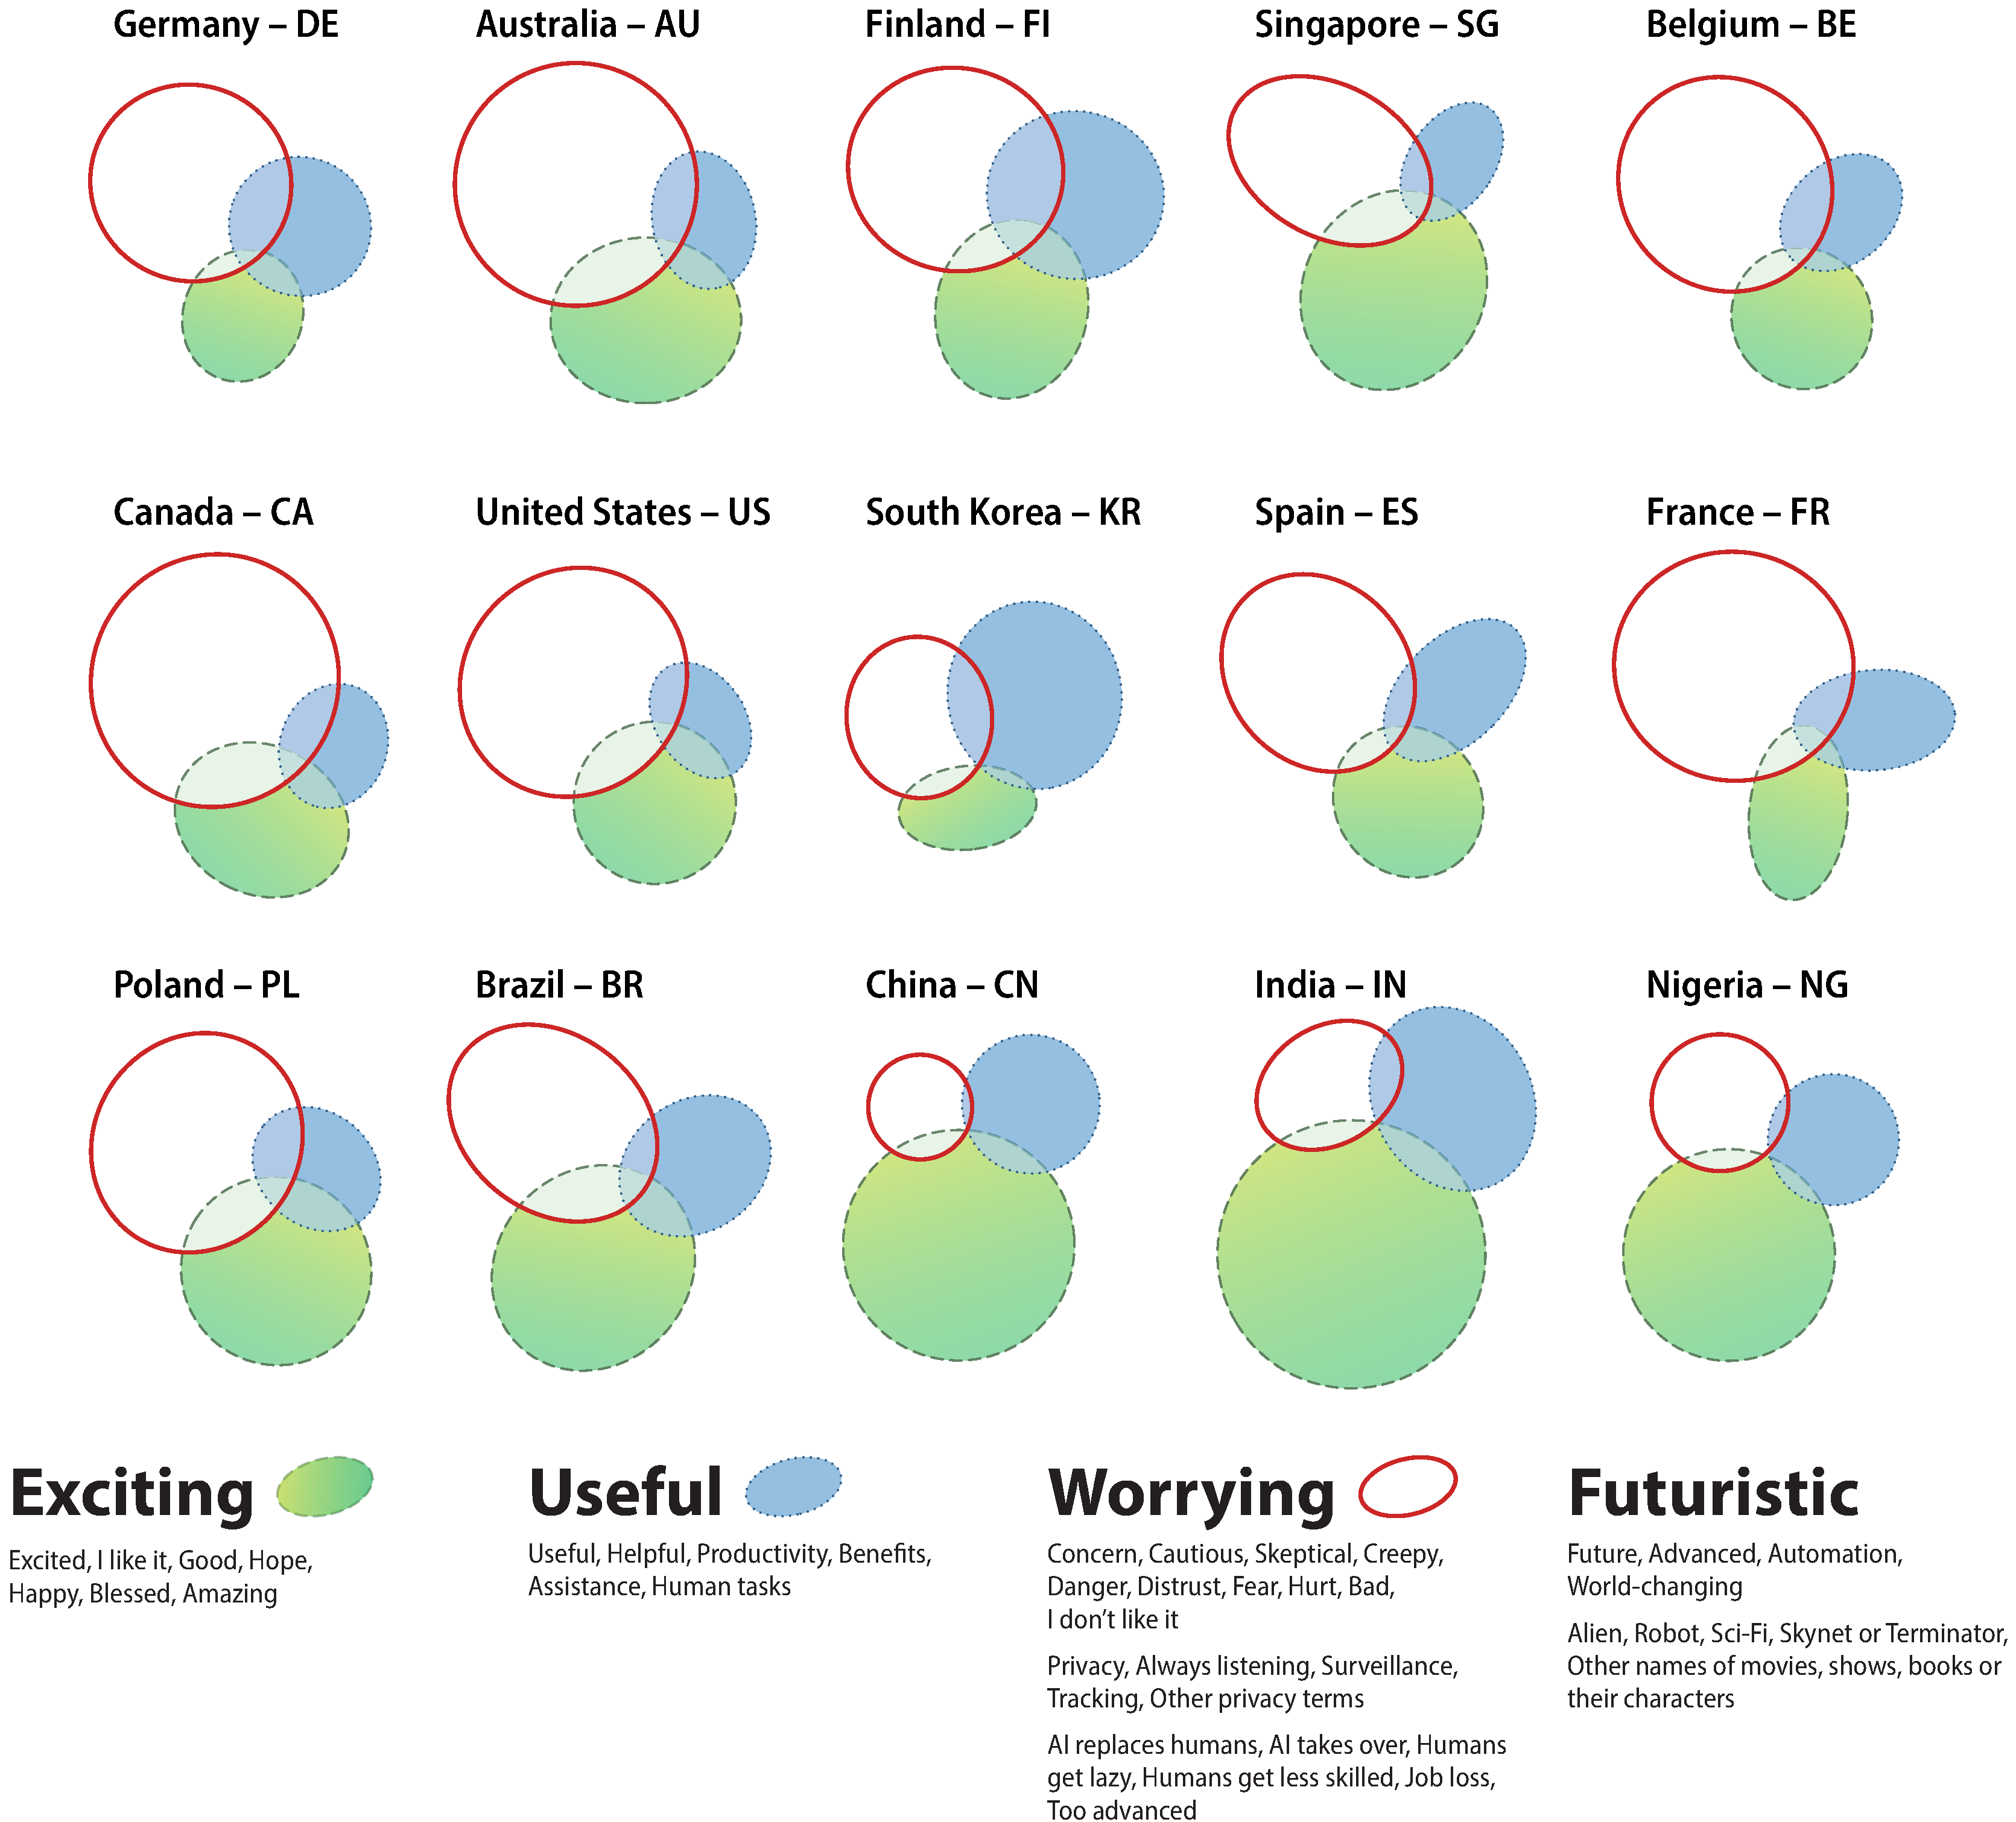
\includegraphics[width=0.95\textwidth]{figs/Rplot09.pdf}
\vspace{-0.3cm}
\setlength\columnsep{12pt}
\begin{multicols}{4}

% EXCITING

\begin{lq1}
%\item \Exciting/
\item excitement for what it can do to simplify and enrich our lives \aff{Canada}
\item Amazing technology that helps us out with everyday mundane things. \aff{US}
\item Happiness, joy from the heart, is to feel that life is convenient \aff{China}
\item joy! The future is now! \aff{Belgium}
\item Happy when I hear this word this can change entire world \aff{India}
\item Great feelings, like the world is moving into a new realm \aff{Nigeria}
% \item I am glad that I am living in a time of such progress. I have high hopes for the development of AI. \aff{Poland}
\end{lq1}

\columnbreak

% USEFUL
\begin{lq1}
%\item \Useful/
\item I have a good feeling! This technology can become useful. \aff{Brazil}
\item A robot that can make people's life more convenient \aff{South Korea}
\item A helpful assistant that is there for us and assists with daily tasks \aff{US}
\item Destined to improve our lives, robotic technology \aff{Spain}
\item Positive, something that makes our lives easier \aff{Poland}
\item The next big efficient thing for humans. \aff{Nigeria}
\end{lq1}

\columnbreak

% WORRYING
\begin{lq1}
%\item \Worrying/ 
\item It is interesting and useful, but I am worried about lost jobs, not to mention AI getting smart enough to take over and control us. \aff{Canada}
\item A little bit of fear because I don't know the limit of Artificial intelligence (if there is a limit) \aff{Nigeria}
% \item This topic is thought-provoking. It generates fear and also curiosity and concern. \aff{Brazil}
\item Progress but danger. Fear, uncertainty. \aff{France}
\item No no no, will ruin everything \aff{Finland}
\item Fearful of our future robot overlords \aff{Australia}
\end{lq1}

\columnbreak

% FUTURE figure
\begin{lq1}
%\item \Futuristic/ (not pictured)
\item Artificial intelligence is the future. It will bring the dawn of a new age \aff{Nigeria}
\item It is the technology that forms the foundation of lives in the next century. \aff{Singapore}
\item A dystopian future, in a way. \aff{Finland}
\item This is the future, personally I don't think it's developing well \aff{Germany}
% \item I try to make an effort to follow this futuristic trend. I really like it and I am onboard with AI in general sense. \aff{Brazil}
\item its magnificient technology of tomorrow \aff{India}
\end{lq1}

\end{multicols}

  \vspace{-0.4cm}
  \caption{\small{Description of our four sentiment groups, with the complete list of codes that comprises each, and example responses. While we use the responses to illustrate a particular sentiment, some of them fall in multiple sentiment groups, as sometimes occurred in our data set. At the top of the figure, we represent the overlap between the groups with Venn diagrams, using 3-Venn diagrams which exclude Futuristic for readability. The alert reader may wonder why we use oblong circles; these more accurately represent the area in the overlap. We use the method described in \protect\cite{micallef2014eulerape}. Countries are ordered by HDI.}}
  \label{fig:venn}
\end{figure*}


Figure~\ref{fig:venn} and Table~\ref{tab:sentimentgroups} present the prevalence of sentiment groups in each country. We now discuss each sentiment in turn.


\subsection{Exciting}

Responses in this group contained positive feelings about AI and often exhibited broad excitement or enthusiasm. These feelings were often direct statements of excitement, but also included other positive feelings such as joy or a sense of feeling blessed to have AI. \Exciting/ sentiment was often associated with a sense of newness or expectation of substantial change. Sometimes respondents expressed excitement about improvements in daily life, and sometimes they anticipated broad improvement for humanity.

\begin{lq2}
\item Excited to see where this tech goes in future, hope to see AI assist with everyday life in the home and in work \aff{Australia}\footnote{Throughout the paper, we share complete verbatim responses (in some cases translated) and do not correct typographic or grammatical errors. The only exception is the quote in the title, which is a verbatim excerpt from a response that is shared in full in Section~\ref{Mixed_Section}.}
\item Happiness, because it means humanity moves forward. \aff{Spain}
\item A bit of excitement, fascination, curiosity, but also somewhere deep a feeling of uncertainty, a thrill related to the effect that it may have on my future, however, that is mostly due to the influence of film rather than a result of conscious assessment of the benefits that AI will bring. \aff{Poland}
\end{lq2}

Some respondents were also excited about potential economic advantages for their country, and a few mentioned personal career opportunities that AI might provide.


\begin{table*}[t]\centering
% \ra{1.3}
\footnotesize
\begin{tabular}{@{}l@{\hskip 0.3cm}rrrrrrrrrrrrrrr@{}}

\emph{Country} & \bf DE & \bf AU & \bf FI & \bf SG & \bf BE & \bf CA & \bf US & \bf KR & \bf ES & \bf FR & \bf PL & \bf BR & \bf CN & \bf IN & \bf NG \\

\midrule
Respondents  & 1002 & 1000 & 1002 & 1000 & 1000 & 1500 & 1501 & 1000 & 1002 & 1001 & 1000 & 1503 & 1003 & 1500 & 1000 \\
($n$) \graynew{\emph{All}} \\
\midrule
\Exciting/ &     9\% & 17\% & 14\% & 22\% & 12\% & 14\% & 15\% &  6\% & 14\% & 10\% & 25\% & 23\% & 28\% & 36\% & 25\% \\
\Useful/ &      12\% &  9\% & 17\% &  7\% &  9\% &  9\% &  7\% & 19\% & 13\% & 11\% & 13\% & 14\% & 13\% & 17\% & 11\% \\
\Worrying/ &    23\% & 31\% & 25\% & 20\% & 27\% & 33\% & 30\% & 14\% & 23\% & 31\% & 30\% & 21\% &  7\% & 9\% &  11\% \\
\Futuristic/ &  17\% & 22\% & 24\% & 21\% & 15\% & 21\% & 19\% & 38\% & 28\% & 20\% & 22\% & 34\% & 24\% & 24\% & 19\% \\
\None/ &        48\% & 38\% & 36\% & 38\% & 48\% & 39\% & 42\% & 31\% & 34\% & 39\% & 32\% & 25\% & 37\% & 27\% & 41\% \\

\bottomrule
\vspace{0.01cm}

\end{tabular}
% \captionof{table}{
\caption{Weighted percentage of respondents from each country whose open-ended sentiment was coded to be in one of our groups. Respondents can appear in multiple sentiment groups. A respondent whose answers received only codes not in these groups appears in \None/.}
\label{tab:sentimentgroups}

\end{table*}

% India really is 17\% useful, even though the AIES paper says 18\%


\subsection{Useful}
Responses in this group expressed the belief that AI will be helpful and assist humans in completing tasks. \Useful/ sentiment was generally associated with practical implications of AI. For example, respondents spoke of AI improving productivity in industrial settings. They also spoke of AI providing personal convenience, making people's lives easier and more comfortable, assisting with daily life, enabling smart home technology, and helping people perform mundane tasks.

\begin{lq2}
\item It is a kind of high technology that brings great convenience to our lives. \aff{China}
\item A tool of the future to make everyday life easier \aff{Finland}
\item Replaces man in thankless tasks \aff{Belgium}
\end{lq2}

Respondents also spoke of AI helping humanity by addressing large societal issues such as healthcare or the environment.
\begin{lq2}
\item Really interesting. Hopefully it can solve energy issues and other large problems. \aff{Finland}
\item Progress, I know it will impact positively especially in the areas of health care.~\aff{Nigeria}
\end{lq2}

\subsection{Worrying}
Many respondents shared that AI is \Worrying/, causing them concern, fear, or anxiety. Unlike the previous two groups, which each capture a relatively tight set of responses to AI in our open-ended data, this group comprises a wide range of negative emotional responses.
\begin{lq2}
\item Do we need that? It scares me! \aff{Germany}
\item A dangerous game. \aff{Finland}
\item It's progress, but I am not sure that it is so positive for society \aff{Belgium}
\end{lq2}

While some respondents spoke of general concerns, many spoke to specific aspects of AI they found \Worrying/. For example, some respondents were concerned that AI might challenge humans and take over society. Sometimes they suggested that popular culture had caused this concern. Correspondingly, they sometimes also spoke to the need for humans to control AI.
\begin{lq2}
\item A threat to the future of humanity. \aff{Finland}
\item regret, it will make work and then the world disappear \aff{Belgium}
\item Can improve or end our lives. \aff{Germany}
\item A mixture of knowledge and fear. I know that it will help or is already helping in several important areas, but there is always that fear that one of these AIs will become too autonomous and turn against us.~\aff{Brazil}
\item That was always coming. But because of all those films on TV with the AI, I still have my reservations. I mean you never know, right? \aff{Belgium}
\item Does no one watch movies, read, or anything to do with science fiction!!! It ALWAYS ends badly... there is just no good outcome, that I can see (for now at least), to an actual, fully fledged, AI.~\aff{US} 
\end{lq2}

Respondents also saw privacy concerns as a likely downside of AI. Sometimes they mentioned privacy in broad terms, but they often raised specific concerns such as worrying that products constantly listen to them, or concerns about being surveilled in the workplace.
\begin{lq2}
\item A new frontier. Very exciting and scary at the same time. Lots to gain but will personal privacy be the price?~\aff{Australia}
\item Could lead to total surveillance \aff{Germany}
\item A trending mobile app that undresses people. It violates privacy rules~\aff{Nigeria}
\item IT DICTATED MY WEIGHT AND HEIGHT IN PUBLIC.~\aff{India}
\item Installing a monitoring system in the office makes people very uncomfortable \aff{China}
\item Ads that show up on computers after visiting websites is one thing, but ads that show up after just talking about something makes me think my phone is listening in on my conversations~\aff{US}
\item The phone's microphone recognizes speech and this information is used in marketing. Should I dare speak about sensitive matters near the phone at all \aff{Finland}
\end{lq2}

Respondents expected that AI would negatively impact the number of jobs available in the future. They perceived that AI may replace humans or make them less necessary in the workforce, and particularly  associated robots with job loss due to their ability to perform human tasks. In rare cases, respondents shared personal experiences with automation-related job loss.
\begin{lq2}
\item I feel that it has taken away jobs~\aff{US}
\item A highly computerised potentially dangerous job stealing system of machinery operation~\aff{Australia}
\item New technologies. Convenience in life. Reduction in jobs.~\aff{South Korea}
\item Am happy about it but am still sceptical about it. This is because it might probably put some persons out of work~\aff{Nigeria}
\item Unemployment comes to my mind when I hear the phrase Artificial Intelligence(AI).~\aff{India}
\end{lq2}

Respondents also expressed concern that humans will become over-reliant on AI and become lazy, or that AI will minimize human contact and negatively impact personal relationships in the future.

\begin{lq2}
\item This is a futuristic innovation that can help people but also make them too lazy~\aff{Nigeria}
\item fear that during my lifetime I will be interacting more with AI than live humans~\aff{US}
\item It helps the future by making things easier, but diminishes employment and human contact.~\aff{France}
\end{lq2}

\subsection{Future}
Although \Futuristic/ may not traditionally be seen as a sentiment, when we asked respondents to describe their feelings or emotions about AI, they organically responded at very high rates and it was clearly a strong association
(15\% to 38\% across the countries).
Responses in this group are not necessarily positive or negative towards AI,
but rather are included for any mention of the futuristic nature of AI, whether by simply describing AI as advanced; mentioning robots, aliens, or other science-fiction concepts; or by referencing the future directly.

Some respondents who spoke of the future expressed that AI will be transformative, for example saying that it will usher in a new era and profoundly change society.
\begin{lq2}
\item Something new. Something that will change the world \aff{Poland}
\item AI can change every aspect of human life. \aff{Singapore}
\item we are entering a new era. Very modern~\aff{Canada}
\item AI will revolutionise the way we live in our future.~\aff{India}
\end{lq2}

The expected future effects of AI were sometimes described as \Exciting/, \Useful/, \Worrying/, or some combination of these. We discuss mixed feelings further below.
\begin{lq2}
\item A thing of the future that is sure to be of great use! \aff{Finland}
\item Better future \aff{Spain}
\item A big problem for humanity in the future. \aff{Poland}
\item Machines taking over humans!! :) on a serious note, A.I. is making things possible we thought were not possible a few years ago. Computers recognise faces and fingerprints of humans. Machines carry out so many things to assist humans. Everywhere we look there are examples of artificial intelligence around us.~\aff{Australia}
\item AI is the new trend for technology, I myself being a tech geek i know that AI is soon going to change the whole world with it's endless possibilities. AI is the future of Mankind \aff{India}
\end{lq2}




\begin{table*}\centering
\footnotesize
\begin{tabular}{@{}l rrrrr rrrrr rrrrr @{}}

Country	&	\bf DE	&	\bf AU	&	\bf FI	&	\bf SG	&	\bf BE	&	\bf CA	&	\bf US	&	\bf KR	&	\bf ES	&	\bf FR	&	\bf PL	&	\bf BR	&	\bf CN	&	\bf IN	&	\bf NG		\\
	
	\midrule
												
Respondents 	&	1002	&	1000	&	1002	&	1000	&	1000	&	1500	&	1501	&	1000	&	1002	&	1001	&	1000	&	1503	&	1003	&	1500	&	1000				\\
	($n$) \graynew{\emph{All}} \\
	\midrule
													
Neutral	&	31\%	&	24\%	&	9\%	&	24\%	&	28\%	&	26\%	&	27\%	&	14\%	&	25\%	&	25\%	&	21\%	&	11\%	&	28\%	&	9\%	&	9\%	\\
I don't know 	&	16\%	&	17\%	&	19\%	&	5\%	&	19\%	&	15\%	&	9\%	&	8\%	&	15\%	&	17\%	&	8\%	&	11\%	&	1\%	&	4\%	&	3\%	\\
Other	&	12\%	&	7\%	&	10\%	&	6\%	&	9\%	&	7\%	&	10\%	&	14\%	&	12\%	&	9\%	&	11\%	&	9\%	&	9\%	&	15\%	&	19\%	\\
Inarticulate	&	15\%	&	5\%	&	12\%	&	10\%	&	12\%	&	7\%	&	6\%	&	4\%	&	6\%	&	19\%	&	8\%	&	4\%	&	7\%	&	7\%	&	4\%	\\
Curious	&	3\%	&	9\%	&	8\%	&	6\%	&	5\%	&	7\%	&	6\%	&	2\%	&	10\%	&	5\%	&	22\%	&	16\%	&	16\%	&	5\%	&	7\%	\\
Intelligence	&	1\%	&	4\%	&	5\%	&	9\%	&	6\%	&	3\%	&	7\%	&	10\%	&	5\%	&	2\%	&	3\%	&	9\%	&	7\%	&	13\%	&	18\%	\\
Technology	&	3\%	&	4\%	&	6\%	&	2\%	&	2\%	&	6\%	&	5\%	&	5\%	&	7\%	&	3\%	&	3\%	&	12\%	&	11\%	&	11\%	&	10\%	\\
Fake	&	1\%	&	3\%	&	4\%	&	3\%	&	4\%	&	4\%	&	7\%	&	3\%	&	2\%	&	1\%	&	4\%	&	2\%	&	0\%	&	6\%	&	17\%	\\
Computer	&	3\%	&	4\%	&	5\%	&	6\%	&	3\%	&	4\%	&	7\%	&	4\%	&	2\%	&	3\%	&	2\%	&	5\%	&	1\%	&	5\%	&	6\%	\\
Device	&	1\%	&	3\%	&	4\%	&	4\%	&	1\%	&	3\%	&	2\%	&	12\%	&	3\%	&	2\%	&	3\%	&	3\%	&	1\%	&	9\%	&	6\%	\\

\bottomrule
\vspace{0.01cm}
\end{tabular}

\caption{ The 10 most common codes within the \None/ group, which includes all respondents who were assigned none of the codes in our four sentiment groups. Weighted percentages indicate how many respondents within the \None/ group were assigned a given code, by country. }
\label{tab:nones}

\end{table*}




\subsection{None}
The groups above do not cover all responses.
Some responses were assigned only the 49 codes that we did not include in our sentiment groups, in which case they fell into the \None/ group described in Section~\ref{Coding_Section}.
These included, for example, broad mentions of technology (responses such as ``technology'' or ``computer''). See Table~\ref{tab:nones}.

\subsection{Mixed Feelings}\label{Mixed_Section}
As seen above, a given response sometimes contained multiple sentiments toward AI. In some responses, these were all positive sentiments, for example, excitement that AI would be helpful in daily life. However, a number of responses were more ambivalent. Sometimes such responses contrasted specific positive expectations (e.g. personal convenience or improved healthcare) with specific negative expectations (e.g. reduced privacy or job loss). Additionally, these mixed emotions were sometimes coupled with a sense of resignation or inevitability. 

\begin{lq2}
\item It is a wonderful and terrifying concept that is inevitable.~\aff{Australia}
\item The future of our world in a way that represents both progress and destruction~\aff{Canada}
\item optimistic that it will enhance peoples lives and bring about breakthroughs in many fields but also skeptical that people will lose their jobs and there will be an invasion of privacy~\aff{Canada}
\item Life will be much more enjoyable, but I fear that we'd lost what makes us human. Robots will replace humans in various fields, but there are positive sides as well, a pet robot being one of them.~\aff{South Korea}
\item I think people are afraid of it and it is the future \aff{Spain}
\item Artificial intelligence is something most people will come to depend on in a few decades. It will make life easier at the same time make people lose their jobs. But one I'm certain of is that AI is here to stay for good.~\aff{Nigeria}
\end{lq2}

Some respondents suggested that the eventual impact of AI is not yet determined, and that multiple outcomes are possible.

\begin{lq2}
\item Both a threat and an opportunity at the same time. \aff{Finland}
\item Mixture of amazement at the potential of this technology and concern about possible pitfalls. Could be the start of something amazing or the beginning of the end (a la Terminator).~\aff{Australia}
\item Unsure about the net value - has lots of positives but also there are some very legitimate concerns.~\aff{Canada}
\item It's exciting to think about the things that could come about with AI that would make our lives easier and safer, but also scary of course, who knows how it will truly effect society~\aff{US}
\end{lq2}

Some respondents also indicated that the effects of AI depend on how it is used, as well as who is using it.

\begin{lq2}
\item Artificial intelligence worries me a bit because if it's not used well it can be dangerous, it has no conscience or ethics, but I acknowledge that it is an amazing tool.~\aff{France}
\item A bit excited because it makes job quite easy but again its scary if it the technology goes wrong like someone using it for evil purposes.~\aff{Nigeria}
\item Artificial Intelligence is very useful for whole human world. But don't use it in a bad way~\aff{India}
\end{lq2}

Some respondents also spoke directly to responsible development of technology. For example, they emphasized the need to think about potential impacts of technology prior to development, or the need for regulation or ethical evaluation.

\begin{lq2}
\item Angry that future concerns or negative impacts aren't ever considered before technology is developed~\aff{Australia}
\item It’s a positive thing, but it needs to be regulated. \aff{Belgium}
\item Unstoppable, but it requires technology ethics \aff{China}
\end{lq2}

\subsection{Country-Level Observations}
We now turn to country-level observations, where we see strikingly different national patterns in response towards AI across the fifteen countries we studied. We visually represent the character of these differences in Figure~\ref{fig:venn}.

\begin{figure*}[t]
\centering
  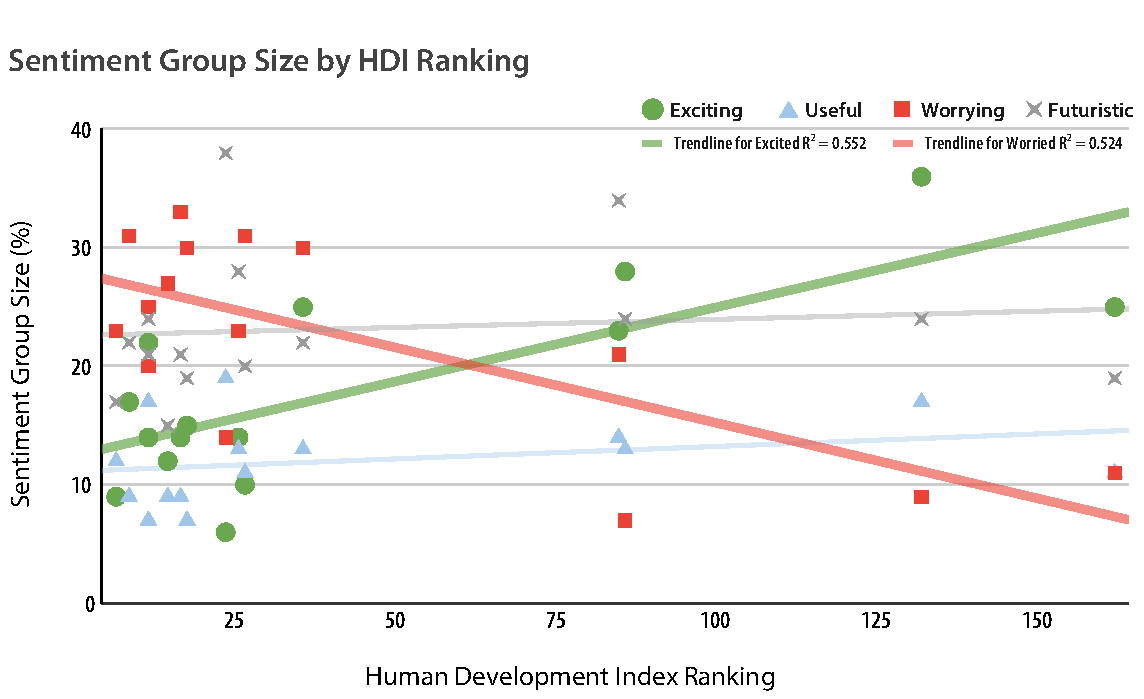
\includegraphics[width=0.7\textwidth]{figs/sentimentbyHDI.pdf}
  \vspace{-0.3cm}
  \caption{Scatter plot of weighted sentiment group size for each country, by HDI rank of the country. Trendlines shown for all four sentiment groups, with \Exciting/ at $R^2 = 0.552$ and \Worrying/ at $R^2 = 0.524$. }
  \label{fig:scatter}
\end{figure*}

Consistent with our expectation that developed countries (those most-developed, by HDI rank) would share similarities, the dominant sentiment groups in Germany, Australia, Finland, Belgium, Canada, the US, and France were \Worrying/ followed by \Futuristic/ (see Table~\ref{tab:sentimentgroups}). Spain had the same two dominant sentiments, although with \Futuristic/ followed by \Worrying/.
This resonates with claims that popular press and media narratives in Western, English-speaking regions have emphasized potential threats of AI~\cite{cave2018portrayals, fast2017long, horvitz2012interim}.

By contrast, we see respondents in developing countries tend to take a more optimistic view of AI's future effects. Respondents in China, India, and Nigeria were least likely to describe AI as \Worrying/ and more likely to describe it as \Exciting/.

Singapore, Poland, and Brazil followed a different pattern, with more balanced numbers of \Worrying/ and \Exciting/.

We can see this relationship more directly in Figure~\ref{fig:scatter} where \Exciting/ and \Worrying/ show clear trends with HDI rank. \Futuristic/ and \Useful/ however do not seem to have a relationship with HDI, highlighting that the development of a country is just one factor in how public opinion towards AI is shaped.

South Korea has a unique profile among the countries surveyed, having the largest percentage in the both the \Useful/ (19\%) and \Futuristic/ (38\%) sentiment groups. South Korean respondents also had the lowest percentage of \Exciting/ (6\% versus 9-36\% in all other countries).
These findings are consistent with South Koreans' high level of exposure to technology: South Korea boasts the world's highest robot density~\cite{ifr2018}, is one of the largest global investors in smart buildings~\cite{ducker2019}, and may be ``at the vanguard of a revolution in AI and big data healthcare''~\cite{nature2019}. Consistent with this, South Korean respondents often mentioned AI assistants and home automation, which may contextualize AI as a more familiar, everyday technology:

\begin{lq2}
\item AI is everywhere from hospitals to homes and cars.~\aff{South Korea}
\item Use big data to make daily life more convenient.~\aff{South Korea}
\item With just the smartphone, I can check the gas, temperature, and the foods in the fridge.~\aff{South Korea}
\item Self-driving car, automated production, convenient daily life~\aff{South Korea}
\end{lq2}


\section{Discussion and Outlook}
We conducted a large-scale investigation of sentiment towards AI across a range of countries. Rather than presupposing particular sentiment, we began with open-ended responses and looked for emergent themes. Our findings revealed sentiment groups as a distinguishing feature, with respondents in different countries finding AI to be \Exciting/, \Useful/, \Worrying/, and \Futuristic/ to varying degrees. These groups provide one nuanced alternative to understanding people's feelings towards AI, rather than considering their orientation to AI as simply positive or negative. While some of these themes have been seen in other literature, here we have documented them occurring unprompted in 15 countries and added richer detail about the sentiment and the mechanisms which inspire this sentiment.

The spontaneously generated open-ended responses reflect a number of key dialogues that have appeared in public discussions and the media~\cite{cave2018portrayals,chuan2019,stone2016artificial,ouchchy2020}, for example, that AI offers significant improvements for health; that AI is associated with privacy issues, job loss, and social isolation; and that AI could be either a significant boon or a significant threat to humanity. The data provide some indication of the ways in which these concepts, as well as different sources of information  (e.g. fiction, news reports, or personal experience) influence sentiment.

This suggests many fruitful avenues for further exploration. For example, it would be valuable to more formally measure and analyze the relationship between media and pop culture narratives in different countries and the presence of these sentiment groups, as well as tracing the relationship and movement of narratives across countries. Further, it would be useful to explore other factors that likely influence these sentiment groups, such as country culture and economy; institutional trust~\cite{chen2020,zhang2022}; presence, awareness, and availability of AI technologies such as customer service chatbots, personal assistants, and more; and personal, formative experiences using AI technology. It would also be worthwhile to explore how sentiment groups affect behavior such as adoption of AI technologies and public opinion on topics such as research funding and regulation.

Public opinion has the potential to shape (and be shaped by) technology development processes and decisions. For example, public opinion can affect whether the public supports research funding for AI. As another example, a negative opinion of a particular technology may discourage consumers from purchasing it. Conversely, new product offerings that rely on AI may influence the public's opinion of AI.

While public opinion can be a beneficial influence, it has also been argued that in some cases it can have suboptimal effects. For example, public misperception or unrealistic expectations of AI may lead to unfounded fears or disappointment, resulting in unwarranted rejection of technology or a lack of support for public funding~\cite{blumberg2019, cave2018portrayals}. But how might one characterize the ``legitimacy'' of public opinion, and to what extent is such characterization a meaningful endeavor? Many issues related to AI are complex questions on which even experts can disagree. And even if experts are in alignment with each other, but not with public opinion, the public may be considering perspectives or values not taken into account by experts~\cite{zhang2022}. It is therefore a complex question how best to interpret or engage with public opinion on a given issue, or whether it might be helpful to influence it. In some cases it may be beneficial to provide the public additional information, while in others it may be more beneficial for researchers and developers to shift the perspectives and values driving the development of AI.

Possible interventions might include educational efforts in areas in which the public may benefit from additional information. Beyond that, however, our findings align with calls to develop technology that supports public values. For example, many respondents were concerned about negative impacts of AI on privacy, reinforcing the value of continued emphasis on designing and developing AI with privacy in mind, concordant with discussion of privacy by design in the EU General Data Protection Regulation (GDPR).\footnote{\url{https://eugdpr.org/}} The privacy discussion continues to evolve quickly, and best practices for AI technologies continue to be actively explored in the academic, legal, and policy communities, offering many opportunities for advances in this area. Further, our findings also suggest ways in which the design and development of particular technologies may have a favorable impact on public opinion.  For example, our findings point to the value of emphasizing AI's application to healthcare in product and research investments as well as communications. As another example, future research could explore the conditions facilitating South Korea's unusually strong impression of AI as \Useful/, to gain insight into whether or how this sentiment might resonate elsewhere via communications or technological offerings.


\section*{Acknowledgments}
We thank Dan Altman, Elie Bursztein, Ed Chi, Charina Chou, Jen Gennai, Reena Jana, Jake Lucchi, Ken Rubinstein, and Kurt Thomas for valuable contributions to this work.
We also thank the cApStAn team for their important contributions to linguistic quality and the Ipsos team for their excellent work fielding the survey.

\bibliographystyle{plain}
\footnotesize
\begin{thebibliography}{10}

\bibitem{abrassart2018}
Christophe Abrassart, Yoshua Bengio, Guillaume Chicoisne, Nathalie
  de~Marcellis-Warin, Marc-Antoine Dilhac, Sebastien Gambs, Vincent Gautrais,
  Martin Gibert, Lyse Langlois, Francois Laviolette, Pascale Lehoux, Jocelyn
  Maclure, Marie Martel, Joelle Pineau, Peter Railton, Catherine Regis,
  Christine Tappolet, and Nathalie Voarino.
\newblock Montreal declaration for responsible development of artificial
  intelligence, 2018.

\bibitem{arm2017}
{ARM | Northstar}.
\newblock {AI} today, {AI} tomorrow. awareness and anticipation of {AI}: A
  global perspective, 2017.

\bibitem{barabas2018}
Chelsea Barabas, Madars Virza, Karthik Dinakar, Joichi Ito, and Jonathan
  Zittrain.
\newblock Interventions over predictions: Reframing the ethical debate for
  actuarial risk assessment.
\newblock In {\em Proceedings of the Conference on Fairness, Accountability,
  and Transparency}, pages 62--76, 2018.

\bibitem{beyer1997contextual}
Hugh Beyer and Karen Holtzblatt.
\newblock {\em Contextual Design: Defining Customer-centered Systems}.
\newblock Elsevier, 1997.

\bibitem{biemer2008weighting}
Paul~P. Biemer and Sharon~L. Christ.
\newblock Weighting survey data.
\newblock In Edith~D. de~Leeuw, Joop~J. Hox, and Don~A. Dillman, editors, {\em
  International Handbook of Survey Methodology}, pages 317--341. Lawrence
  Erlbaum Associates New York, NY, 2008.

\bibitem{blumberg2019}
{Blumberg Capital}.
\newblock Artificial intelligence in 2019: Getting past the adoption tipping
  point, 2019.

\bibitem{brynjolfsson2014second}
Erik Brynjolfsson and Andrew McAfee.
\newblock {\em The Second Machine Age: Work, Progress, and Prosperity in a Time
  of Brilliant Technologies}.
\newblock WW Norton \& Company, 2014.

\bibitem{bucher2017algorithmic}
Taina Bucher.
\newblock The algorithmic imaginary: exploring the ordinary affects of
  {F}acebook algorithms.
\newblock {\em Information, Communication \& Society}, 20(1):30--44, 2017.

\bibitem{buolamwini2018}
Joy Buolamwini and Timnit Gebru.
\newblock Gender shades: Intersectional accuracy disparities in commercial
  gender classification.
\newblock In {\em Proceedings of the Conference on Fairness, Accountability,
  and Transparency}, pages 77--91, 2018.

\bibitem{castro2019}
Daniel Castro.
\newblock The {U}.{S}. may lose the {AI} race because of an unchecked
  techno-panic.
\newblock {\em Center for Data Innovation}, March 2019.

\bibitem{cave2019}
Stephen Cave, Kate Coughlan, and Kanta Dihal.
\newblock ``{S}cary {R}obots'': Examining public responses to {AI}.
\newblock In {\em Proceedings of the 2019 AAAI/ACM Conference on AI, Ethics,
  and Society (AIES 2019)}, pages 331--337, 2019.

\bibitem{cave2018portrayals}
Stephen Cave, Claire Craig, Kanta~Sarasvati Dihal, Sarah Dillon, Jessica
  Montgomery, Beth Singler, and Lindsay Taylor.
\newblock {\em Portrayals and perceptions of {AI} and why they matter}.
\newblock The Royal Society, 2018.

\bibitem{cave2020narratives}
Stephen Cave, Kanta Dihal, and Sarah Dillon.
\newblock {\em {AI} Narratives: A History of Imaginative Thinking about
  Intelligent Machines}.
\newblock Oxford Scholarship Online, 2020.

\bibitem{cbs2016}
{CBS News}.
\newblock 60 {M}inutes/{V}anity {F}air poll: Artificial intelligence, March
  2016.

\bibitem{princetonEthics}
{Center for Information Technology Policy} and {University Center for Human
  Values}.
\newblock Princeton dialogues on {AI} and ethics case studies.
\newblock \url{https://aiethics.princeton.edu/case-studies}.

\bibitem{chancellor2019}
Stevie Chancellor, Michael~L. Birnbaum, Eric~D. Caine, Vincent M.~B. Silenzio,
  and Munmun De~Choudhury.
\newblock A taxonomy of ethical tensions in inferring mental health states from
  social media.
\newblock In {\em Proceedings of the Conference on Fairness, Accountability,
  and Transparency}, page 79–88, 2019.

\bibitem{chen2020}
Yi-Ning Chen and Chia-Ho Wen.
\newblock Impacts of attitudes toward government and corporations on public
  trust in artificial intelligence.
\newblock {\em Communication Studies}, 72(1):115--131, 2020.

\bibitem{chuan2019}
Ching-Hua Chuan, Wan-Hsiu Tsai, and Su~Cho.
\newblock Framing artificial intelligence in {A}merican newspapers.
\newblock In {\em Proceedings of the 2019 AAAI/ACM Conference on AI, Ethics,
  and Society (AIES 2019)}, pages 339--344, 2019.

\bibitem{devito2017platforms}
Michael~A. DeVito, Jeremy Birnholtz, and Jeffery~T. Hancock.
\newblock Platforms, people, and perception: Using affordances to understand
  self-presentation on social media.
\newblock In {\em Proceedings of the 2017 ACM Conference on Computer Supported
  Cooperative Work and Social Computing}, pages 740--754, 2017.

\bibitem{dietterich2015rise}
Thomas~G. Dietterich and Eric Horvitz.
\newblock Rise of concerns about {AI}: Reflections and directions.
\newblock {\em Communications of the ACM}, 58(10):38--40, 2015.

\bibitem{ducker2019}
DuckerFrontier.
\newblock Smart building trends in 2019: Part 1, April 2019.

\bibitem{dutton2018}
Tim Dutton.
\newblock An overview of national {AI} strategies.
\newblock {\em Medium}, June 2018.

\bibitem{edelman2019}
Edelman.
\newblock 2019 {E}delman {AI} survey, March 2019.

\bibitem{eslami2015always}
Motahhare Eslami, Aimee Rickman, Kristen Vaccaro, Amirhossein Aleyasen, Andy
  Vuong, Karrie Karahalios, Kevin Hamilton, and Christian Sandvig.
\newblock ``{I} always assumed that {I} wasn't really that close to [her]'':
  Reasoning about invisible algorithms in news feeds.
\newblock In {\em Proceedings of the 33rd Annual ACM Conference on Human
  Factors in Computing Systems}, pages 153--162, 2015.

\bibitem{fast2017long}
Ethan Fast and Eric Horvitz.
\newblock Long-term trends in the public perception of artificial intelligence.
\newblock In {\em Thirty-First AAAI Conference on Artificial Intelligence},
  2017.

\bibitem{fjeld2020}
Jessica Fjeld, Nele Achten, Hannah Hilligoss, Adam Nagy, and Madhulika
  Srikumar.
\newblock Principled artificial intelligence: Mapping consensus in ethical and
  rights-based approaches to principles for {AI}.
\newblock {\em Berkman Klein Center Research Publication}, 2020.

\bibitem{scuEthics}
Markkula~Center for Applied~Ethics.
\newblock Ethics in technology practice.
\newblock \url{http://www.scu.edu/ethics-in-technology-practice/}.

\bibitem{funk2020}
Cary Funk, Alec Tyson, Brian Kennedy, and Courtney Johnson.
\newblock Science and scientists held in high esteem across global publics.
\newblock {\em Pew Research Center}, September 2020.

\bibitem{garvey2019sentiment}
Colin Garvey and Chandler Maskal.
\newblock Sentiment analysis of the news media on artificial intelligence does
  not support claims of negative bias against artificial intelligence.
\newblock {\em OMICS: a Journal of Integrative Biology}, 2019.

\bibitem{hawking2014}
Stephen Hawking, Max Tegmark, and Frank Wilczek.
\newblock Transcendence looks at the implications of artificial intelligence -
  but are we taking {AI} seriously enough?
\newblock {\em The Independent}, May 2014.

\bibitem{highlevel2019}
{High-Level Expert Group on Artificial Intelligence}.
\newblock Ethics guidelines for trustworthy {AI}, 2019.

\bibitem{hinkin1998brief}
Timothy~R. Hinkin.
\newblock A brief tutorial on the development of measures for use in survey
  questionnaires.
\newblock {\em Organizational Research Methods}, 1(1):104--121, 1998.

\bibitem{holbrook2003telephone}
Allyson~L. Holbrook, Melanie~C. Green, and Jon~A. Krosnick.
\newblock Telephone versus face-to-face interviewing of national probability
  samples with long questionnaires: Comparisons of respondent satisficing and
  social desirability response bias.
\newblock {\em Public Opinion Quarterly}, 67(1):79--125, 2003.

\bibitem{horvitz2012interim}
Eric Horvitz and Bart Selman.
\newblock Interim report from the panel chairs: {AAAI} {P}residential {P}anel
  on long-term {AI} futures.
\newblock In {\em Singularity Hypotheses}, pages 301--308. Springer, 2012.

\bibitem{ethicalOS}
{Institute for the Future} and {Omidyar Network}.
\newblock Ethical {OS} {T}oolkit.
\newblock \url{https://ethicalos.org}.

\bibitem{ifr2018}
{International Federation of Robotics}.
\newblock Robot density rises globally, Feb 2018.

\bibitem{ipsos2019}
Ipsos.
\newblock Widespread concern about artificial intelligence, 2019.

\bibitem{jobin2019}
Anna Jobin, Marcello Ienca, and Effy Vayena.
\newblock The global landscape of {AI} ethics guidelines.
\newblock {\em Nature Machine Intelligence}, 1:389--399, September 2019.

\bibitem{kalyanakrishnan2018opportunities}
Shivaram Kalyanakrishnan, Rahul~Alex Panicker, Sarayu Natarajan, and Shreya
  Rao.
\newblock Opportunities and challenges for artificial intelligence in {I}ndia.
\newblock In {\em Proceedings of the 2018 AAAI/ACM Conference on AI, Ethics,
  and Society (AIES 2018)}, pages 164--170. ACM, 2018.

\bibitem{kelley2021}
Patrick~Gage Kelley, Yongwei Yang, Courtney Heldreth, Christopher Moessner,
  Aaron Sedley, Andreas Kramm, David~T. Newman, and Allison Woodruff.
\newblock Exciting, useful, worrying, futuristic: Public perception of
  artificial intelligence in 8 countries.
\newblock In {\em Proceedings of the 2021 AAAI/ACM Conference on AI, Ethics,
  and Society (AIES '21)}, page 627–637, 2021.

\bibitem{lloyds2020}
{Lloyd’s Register Foundation}.
\newblock World {R}isk {P}oll report 2019, 2020.

\bibitem{mccorduck2004machines}
Pamela McCorduck.
\newblock {\em Machines Who Think}.
\newblock A K Peters/CRC Press, 1979.

\bibitem{mcdonald2019}
Nora McDonald, Sarita Schoenebeck, and Andrea Forte.
\newblock Reliability and inter-rater reliability in qualitative research:
  Norms and guidelines for {CSCW} and {HCI} practice.
\newblock In {\em Proceedings of the 22nd ACM Conference on Computer Supported
  Cooperative Work and Social Computing (CSCW 2019)}, 2019.

\bibitem{micallef2014eulerape}
Luana Micallef and Peter Rodgers.
\newblock {eulerAPE}: drawing area-proportional 3-{V}enn diagrams using
  ellipses.
\newblock {\em PloS one}, 9(7):e101717, 2014.

\bibitem{mozilla2019}
Mozilla.
\newblock We asked people around the world how they feel about artificial
  intelligence. {H}ere's what we learned., 2019.

\bibitem{nature2019}
Nature.
\newblock {AI} and big data healthcare in {K}orea.
\newblock {\em Nature Focal Point}, March 2019.

\bibitem{neudert2020}
Lisa-Maria Neudert, Aleksi Knuutila, and Philip~N. Howard.
\newblock Global attitudes towards {AI}, machine learning \& automated decision
  making: Implications for involving artificial intelligence in public service
  and good governance.
\newblock {\em Oxford Internet Institute}, 2020.

\bibitem{nils2009}
Nils~J. Nilsson.
\newblock {\em The Quest for Artificial Intelligence: A History of Ideas and
  Achievements}.
\newblock Cambridge University Press, 2009.

\bibitem{northeastern2018}
{Northeastern University and Gallup}.
\newblock Optimism and anxiety: Views on the impact of artificial intelligence
  and higher education's response, January 2018.

\bibitem{openAI2019}
OpenAI.
\newblock Better language models and their implications.
\newblock {\em OpenAI Blog}, Feb 2019.

\bibitem{ouchchy2020}
Leila Ouchchy, Allen Coin, and Veljko Dubljevi{\'c}.
\newblock {AI} in the headlines: The portrayal of the ethical issues of
  artificial intelligence in the media.
\newblock {\em AI \& Society}, 35:927--936, 2020.

\bibitem{googleAI}
Sundar Pichai.
\newblock {AI} at {G}oogle: our principles, June 2018.
\newblock \url{http://www.blog.google/technology/ai/ai-principles/}.

\bibitem{rader2015understanding}
Emilee Rader and Rebecca Gray.
\newblock Understanding user beliefs about algorithmic curation in the
  {F}acebook news feed.
\newblock In {\em Proceedings of the 33rd Annual ACM Conference on Human
  Factors in Computing Systems}, pages 173--182, 2015.

\bibitem{raghavan2020}
Manish Raghavan, Solon Barocas, Jon Kleinberg, and Karen Levy.
\newblock Mitigating bias in algorithmic hiring: Evaluating claims and
  practices.
\newblock In {\em Proceedings of the 2020 Conference on Fairness,
  Accountability, and Transparency}, page 469–481, 2020.

\bibitem{salkind2010}
Neil~J. Salkind, editor.
\newblock {\em Encyclopedia of Research Design}, volume~1.
\newblock Sage, 2010.

\bibitem{sambasivan2019toward}
Nithya Sambasivan and Jess Holbrook.
\newblock Toward responsible {AI} for the next billion users.
\newblock {\em Interactions}, 26(1):68--71, 2019.

\bibitem{sanchez-mondero2020}
Javier S\'{a}nchez-Monedero, Lina Dencik, and Lilian Edwards.
\newblock What does it mean to `solve' the problem of discrimination in
  hiring?: Social, technical and legal perspectives from the {UK} on automated
  hiring systems.
\newblock In {\em Proceedings of the 2020 Conference on Fairness,
  Accountability, and Transparency}, page 458–468, 2020.

\bibitem{scharre2018army}
Paul Scharre.
\newblock {\em Army of None: Autonomous Weapons and the Future of War}.
\newblock WW Norton \& Company, 2018.

\bibitem{stone2016artificial}
Peter Stone, Rodney Brooks, Erik Brynjolfsson, Ryan Calo, Oren Etzioni, Greg
  Hager, Julia Hirschberg, Shivaram Kalyanakrishnan, Ece Kamar, Sarit Kraus,
  et~al.
\newblock Artificial intelligence and life in 2030.
\newblock {\em One Hundred Year Study on Artificial Intelligence: Report of the
  2015-2016 Study Panel}, page~52, 2016.

\bibitem{european2017}
{The European Commission}.
\newblock Special {E}urobarometer 460: Attitudes towards the impact of
  digitisation and automation on daily life, May 2017.

\bibitem{un2014}
{United Nations}.
\newblock World economic situation and prospects: Country classification, 2014.

\bibitem{ur2012smart}
Blase Ur, Pedro~Giovanni Leon, Lorrie~Faith Cranor, Richard Shay, and Yang
  Wang.
\newblock Smart, useful, scary, creepy: perceptions of online behavioral
  advertising.
\newblock In {\em Proceedings of the Eighth Symposium on Usable Privacy and
  Security (SOUPS) 2012}, 2012.

\bibitem{warshaw2016intuitions}
Jeffrey Warshaw, Nina Taft, and Allison Woodruff.
\newblock Intuitions, analytics, and killing ants: Inference literacy of high
  school-educated adults in the {US}.
\newblock In {\em Proceedings of the Twelfth Symposium on Usable Privacy and
  Security (SOUPS) 2016}, pages 271--285, 2016.

\bibitem{west2018}
Darrell~M. West.
\newblock Brookings survey finds divided views on artificial intelligence for
  warfare, but support rises if adversaries are developing it.
\newblock {\em Brookings}, August 2018.

\bibitem{wilson2014}
Max~L. Wilson, Ed~H. Chi, Stuart Reeves, and David Coyle.
\newblock Repli{CHI}: The {W}orkshop {II}.
\newblock In {\em CHI Extended Abstracts '14}, page 33–36, 2014.

\bibitem{you2015}
Jia You.
\newblock A 100-year study of artificial intelligence? {M}icrosoft {R}esearch's
  {E}ric {H}orvitz explains.
\newblock {\em Science}, January 2015.

\bibitem{zhang2022}
Baobao Zhang.
\newblock Public opinion toward artificial intelligence.
\newblock In Justin Bullock, Baobao Zhang, Yu-Che Chen, Johannes Himmelreich,
  Matthew Young, Antonin Korinek, and Valerie Hudson, editors, {\em Oxford
  Handbook on AI Governance}. Oxford University Press, 2022.

\bibitem{zhang2019artificial}
Baobao Zhang and Allan Dafoe.
\newblock Artificial intelligence: American attitudes and trends.
\newblock {\em Available at SSRN 3312874}, 2019.

\end{thebibliography}





\normalsize

\section*{Appendix: Select Questions}
\noindent{Note that some questions were modified from or replicate other questions in the literature or the canon of public opinion surveys}. For additional select questions used in the instrument see \href{https://arxiv.org/abs/2001.00081}{arXiv:2001.00081}

\small 

\question{Unaided Sentiment}
\sample{Ask All}
\questiontext{What feelings or emotions come to mind when you hear the phrase Artificial Intelligence (AI)?}
\openend

\question{Knowledge}
\sample{Ask All}
\questiontext{How much do you know about Artificial Intelligence (AI)?}
\begin{itemize}
  \setlength\itemsep{-0.3em}
\item{A lot}
\item{A moderate amount}
\item{A little}
\item{Heard of AI, but know nothing about it}
\item{Never heard of AI}
\end{itemize}

\question{Unaided Description}
\sample{Do NOT ask if ``Never heard of AI'' in Knowledge question}
\questiontext{In your own words, please describe Artificial Intelligence (AI).}
\openend

\question{Unaided Examples}
\sample{Do NOT ask if ``Never heard of AI'' in Knowledge question}
\questiontext{Please list some examples of how Artificial Intelligence (AI) is used today.}
\openend

\question{Uncomfortable Experience}
\sample{Do NOT ask if ``Never heard of AI'' in Knowledge question}
\questiontext{Have you ever had an experience with AI-related technology that made you feel uncomfortable?}
\begin{itemize}
  \setlength\itemsep{-0.3em}
\item{Yes}
\item{No}
\item{Not sure}
\end{itemize}

\question{Unaided Description of Uncomfortable Experience}
\sample{Ask if ``Yes'' to Uncomfortable Experience}
\questiontext{What happened, and what was the outcome? Please describe your experience with AI that made you feel uncomfortable.}
\openend

\vspace{12pt}

\end{document}
